\documentclass[12pt,conference]{IEEEtran}

\usepackage{cite}
\usepackage{amsmath,amssymb,amsfonts}
\usepackage{algorithmic}
\usepackage{graphicx}
\usepackage{textcomp}
\usepackage{xcolor}
\def\BibTeX{{\rm B\kern-.05em{\sc i\kern-.025em b}\kern-.08em
		T\kern-.1667em\lower.7ex\hbox{E}\kern-.125emX}}
	
\begin{document}
	
	\title{Parallel Genetic Programming
	}
	
	\author{\IEEEauthorblockN{Abiyaz Chowhury}

		\and
		\IEEEauthorblockN{Allen Kim}

	}
	
	\maketitle
	
	\begin{abstract}
Genetic programming is a technique in the field of genetic algorithms that evolve computer programs themselves. Programs are encoded in some computational representation that are then run through the standard genetic operations (selection, crossover, mutation). However, the computational cost to train genetic programs grows rapidly as the complexity of the problem increases. We aim to implement a highly parallel version of genetic programming that will scale efficiently.
	\end{abstract}
	
	\begin{IEEEkeywords}
		parallel, genetic, programming
	\end{IEEEkeywords}
	
	\section{Introduction}
	Genetic algorithms have primarily seen use in optimizing numerical parameters. However, genetic programming has not seen as much mainstream use in the past due to its severe computational costs. Genetic programming aims to evolve the computer program themselves over time rather than various function parameters \cite{b1}. By having programs themselves be the population, genetic programming ultimately aims to have computer-generated programs that show distinct characteristics from human written programs and ideally, efficient as well.
	
	The main problem with genetic programming is the fact that in practice, it is only able to solve small problems. The sheer number of possible programs that exist makes it difficult to even create simple programs. However, with the growth in modern computing power and the use of parallelism, genetic programming is beginning to seem more practical.
	
	\section{Prior Work}
	
	One main topic in prior work in genetic programming deals with how to represent the programs themselves structurally. The simplest idea was to use a forest of parse trees since compilers are used to dealing with such structures for programs, but they tend to be much slower to analyze. Other data structures such as directed acyclic graphs \cite{b2} were later proposed to allow for greater efficiency, but we focused on parallel distributed genetic programming (PDGP) \cite{b3}. 
	
	In PDGP, programs are encoded as grids in which each node can be non-terminal or terminal. Non-terminal nodes represent different functions that take in other nodes as arguments while terminal nodes represent the input to the program. There are many variations to the grid, but we chose one of the simplest representations. Akin to a feed forward neural network, we considered grids that had connective edge between adjacent layers. Thus, our programs would propagate values upward from bottom to top through a series of nodes. This was still an efficient representation as nodes can be reused by the layers above, but was also simple enough to understand and implement. With the identity node, any grid could be represented in this way given sufficient rows and columns.
	
	Regarding the parallel implementations of genetic programming, most prior work splits up the population among the processors and evaluate fitness in parallel \cite{b4}. We aimed to implement these core ideas in our program as well.
	
	
	\section{Overview}
	For our project, we implemented a parallelized version of PDGP, which was built to solve arbitrary combinatorial circuit problems. We allow the use of AND, OR, NOT, NAND, NOR, and I (identity) as our non-terminals. We also use $x_1$ to $x_n$ for our input. Given a function we want to learn, we use our program to find circuits that can solve it. We test our program on solving XOR as well as solving the even-3 parity problem. 
	
	\section{Description of Implementation}

	\subsection{Random Graph Generation}
	To initialize the graph, we assume that we are given a set width and height for our grid. Then, we randomly fill the grid with non-terminal and terminal nodes randomly. We do place certain constraints, however. The bottom row of the grid are always restricted to be terminals while the output node at the top is always restricted to be non-terminal. This is to ensure that every grid corresponds to a valid program. By default, each node is inactive, but after initializing, we mark every node connected to the output as active. 
	
	For our random number generator, we use a variant of XOR shifting pseudo random number generators, which run much faster than the rand function in the standard library. This is important to optimize the speed in which our populations are generated.
	\subsection{Evaluation and Fitness}
	
	\subsection{Genetic Operators}
	\subsubsection{Crossover}
	For crossover, there are many variations discussed in Poli’s work on PDGP, but we chose to implement the one that seemed most effective and simplest to implement: sub-sub graph active-active node. In this version of crossover, we first randomly select an active node from the one graph and a random active node from the second graph. Then, we copy the subgraph rooted at the first node over to the second node. We prune off any nodes that may extend beyond the graph as well.
	\subsubsection{Mutation}
	We consider three forms of mutations: global, link, and node. The first two are discussed in Poli’s original work, but the third form was not used. We also implemented it to see if it had any positive effect.
	\begin{itemize}
		\item Global mutation injects a random subgraph at a random active node in the candidate graph. We implemented this by conducting crossover with a randomly generated graph.
		
		\item Link mutation randomly changes an edge in the grid to point to a random node below it.
		
		\item Node mutation randomly changes a node in the grid to become terminal or non-terminal and then, randomly assigns a new function or value to the node.
		
	\end{itemize}
	\subsubsection{Selection}
	For selection, we use tournament selection where the size of tournament is a parameter to the program. In tournament selection, we are given a number of participants, say $k$, and we randomly sample $k$ candidates from the current population. The one with the highest fitness from this set is selected. By varying the tournament size, one can control the selection pressure. If the tournament size is small, then candidates with lower fitness are more likely to survive whereas if the tournament gets larger, then there are more and more possibilities for stronger candidates to go through.
	
	\subsection{Run of a single generation}
For a single generation, we run the following steps:
\begin{enumerate}
\item Run selection twice to find candidates for both parents.
\item With some probability, conduct crossover to create a child grid.
\item With some probability, run global mutation on the child.
\item With some probability, run link mutation on the child.
\item With some probability, run node mutation on the child.
\item Add the child to the new population and repeat steps 1 to 5 until population is full.
\end{enumerate}

	\subsection{Multi-start Evaluation}
	Since genetic programming is not guaranteed to converge to the global best, we also employ a simple technique to try and initialize and run our programs with different seeds. We then take the best fit across all of these programs. This is easily parallelizable since each genetic program can be run independently from one another. 
	
	\section{Results}
	In Figure \ref{xor_scalability}, we show the scalability of the XOR program. This was run on a 3 by 3 grid with a population size of 200 and with 20 generations. The tournament size was 7, and the crossover probability was 0.7. Also, the probability for global, link, and node mutations were all set to be 0.25. Our program successfully discovers new ways to compute XOR with every run.
\begin{figure*}
	\centering
	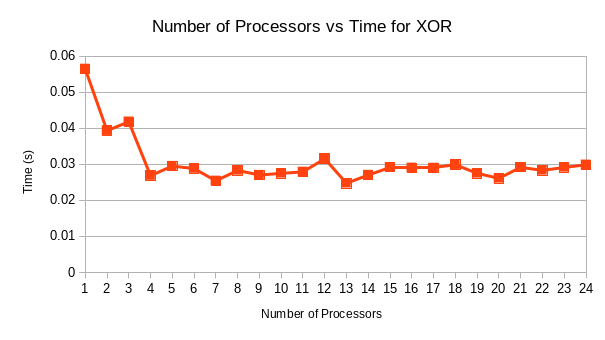
\includegraphics{xor_scalability.png}
	\caption{Scalability of XOR}
	\label{xor_scalability}
\end{figure*}
	
	In Figure \ref{parity_scalability}, we show the scalability of the even-3 parity program. This was run on a 4 by 2 grid with a population size of 2000 and with 50 generations. The tournament size was 30, and the crossover probability was 0.7. Also, the probability for global, link, and node mutations were all set to be 0.05. Our program successfully discovers new ways to compute even-3 parity with every run.

\begin{figure*}
	\centering
	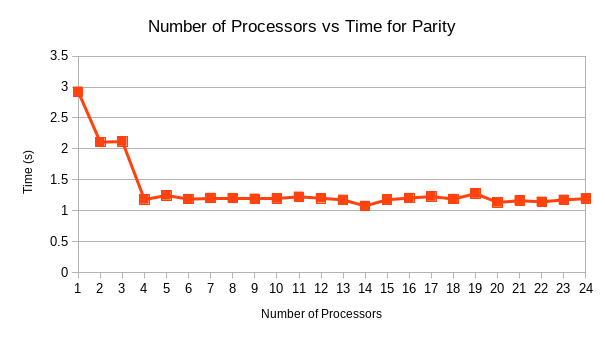
\includegraphics{parity_scalability.png}
	\caption{Scalability of Even-3 Parity}
	\label{parity_scalability}
\end{figure*}
	
	\section{Future Work}
	
	Currently, our approach is restricted to be a feed-forward grid, and as such, we cannot expect to solve any problems that go beyond the scope of a general combinatorial circuit. Ideally, we want to compute general functions. One simple extension would be to compute symbolic regressions, in which our non-terminals would be common mathematical operators, and we would try to deduce what function maps a given set of training points. Another nice expansion would be to use assembly instructions as our non-terminals and have our input nodes accept some string encoding to our program.
	
	We also could try experimenting with different crossover operations. At the moment, 
	
	Additionally, another way to generalize our approach would be to use meta-genetic programming \cite{b5}. Currently, we hard-code in the parameters to our prog
	rams for each example such as the crossover and mutation probabilities or tournament size. In theory, these parameters can also be evolved with our programs. However, it is not clear that this would add much benefit, but can be something to experiment with.
	
	\begin{thebibliography}{00}
				
		\bibitem{b1} McPhee, Nicholas Freitag, Riccardo Poli, and William B. Langdon. Field
		guide to genetic programming. (2008).
		
		\bibitem{b2} S.Handley. On the use of a directed acyclic graph to represent a population of computer programs. In Proceedings of the 1994 IEEE World Congress on Computational Intelligence, pages 154-159, Orlando, Florida, USA, 27-29 June 1994. IEEE Press.

		\bibitem{b3} Poli, Riccardo. Parallel distributed genetic programming. University of Birmingham, Cognitive Science Research Centre, 1996.

		\bibitem{b4} Kilian Stoffel and Lee Spector. High-performance, parallel, stack-based genetic programming. In John R. Koza, David E. Goldberg, David B. Fogel, and Rick L. Riolo, editors, Genetic Programming 1996: Proceedings of the First Annual Conference, page 224, Stanford University, CA, USA, 28-31 July 1996. MIT Press.
			
		\bibitem{b5} B. Edmonds, “Meta-genetic programming: Co-evolving the operators of variation,” CPM Report No.: 98-32. Centre for Policy Modelling, Manchester Metropolitan University. http://www.cpm.mmu.ac.uk/cpmrep32.html, 1998.
		\end{thebibliography}
	
\end{document}
